\documentclass{beamer}

% Customize beamer
\usepackage[absolute, overlay]{textpos} 
\usepackage{color}
\usepackage[T1]{fontenc}
\usepackage[utf8]{inputenc}
\usepackage[danish]{babel}
\usepackage{amssymb}
\usepackage{amsfonts}
\usepackage{amsmath}
\usepackage{algorithm}
\usepackage{setspace}
\usepackage[noend]{algpseudocode}

\usepackage{xspace}
\usepackage{algpseudocode}
\newcommand*\Let[2]{\State #1 $\gets$ #2}
\newcommand*\Returns[1]{\State \Return #1}
\newcommand{\setalglineno}[1]{\setcounter{ALC@line}{\numexpr#1-1}}
\algrenewcommand\algorithmicrequire{\textbf{Input:}}
\algrenewcommand\algorithmicensure{\textbf{Output:}}
\renewcommand{\algorithmicforall}{\textbf{foreach}}
\algnewcommand{\Or}{\textbf{or}\xspace}
\algnewcommand{\Not}{\textbf{not}\xspace}
\algnewcommand{\In}{\textbf{in}\xspace}

%%%%%%%%%%%%%%%%%%%%%%%%%
%          Tikz         %
\usepackage{tikz}
\usepackage{pgfplots}
\pgfplotsset{compat=newest}
\usetikzlibrary{shapes.geometric,arrows,fit,matrix,positioning}
\tikzset
{
    treenode/.style = {align=center, minimum size=1cm},
    subtree/.style  = {isosceles triangle, draw=black, align=center, minimum height=0.5cm, minimum width=1cm, shape border rotate=90, anchor=north}
}

%                       %
%%%%%%%%%%%%%%%%%%%%%%%%%

\setbeamersize{text margin left=15mm} 
\setbeamersize{text margin right=15mm}

\definecolor{kugray}{gray}{0.4}
\definecolor{kured}{rgb}{0.569, 0.094, 0.114}

\setbeamercolor{title}{fg=kured}
\setbeamercolor{frametitle}{fg=kured}
\setbeamercolor{structure}{fg=kured}

\setbeamertemplate{frametitle}{
    
    \color{kured}
    \fontsize{10.5}{14}\selectfont
    \insertframetitle
    \par
}

\setbeamertemplate{navigation symbols}{} % no symbols

\makeatletter

\addtobeamertemplate{headline}{}{

    \ifnum\c@framenumber>1

        \begin{textblock*}{0mm}(115mm , 81mm)
            
\includegraphics[height=13mm, keepaspectratio]{ku/logo}
        \end{textblock*}

        \begin{textblock*}{200mm}(-12mm, 93.0mm)
            \textblockcolour{kured}
            \fontsize{0}{0}\selectfont
            \TPMargin{0mm}
            \vspace{0.1mm}.
        \end{textblock*}

    \fi

    \begin{textblock*}{200mm}(-12mm, 0mm)
        \textblockcolour{kugray}
        \fontsize{0}{0}%\selectfont
        \TPMargin{0mm}
        \vspace{3.3mm}.
    \end{textblock*}

    \begin{textblock*}{115mm}(2mm, 1mm)
        \textblockcolour{}
        \fontsize{4.5}{12}\fontfamily{ttf}\selectfont
        \textbf{\textcolor{white}{
            U N I V E R S I T Y \; O F \; C O P E N H A G E N
        }}
    \end{textblock*}

    \begin{textblock*}{50mm}(89mm, 1mm)
    \textblockcolour{}
    \fontsize{4.5}{12}\fontfamily{ttf}\selectfont
    \textbf{\textcolor{white}{
            C O M P U T E R \; S C I E N C E
    }}
    \end{textblock*}

    \vskip+12mm

}

\defbeamertemplate*{title page}{customized}[1][]
{

    %\begin{textblock*}{0mm}(80mm , 48mm)
    %    \includegraphics[height=50mm, keepaspectratio]{title}
    %\end{textblock*}

    
    \begin{textblock*}{0mm}(67.5mm , 22mm)
        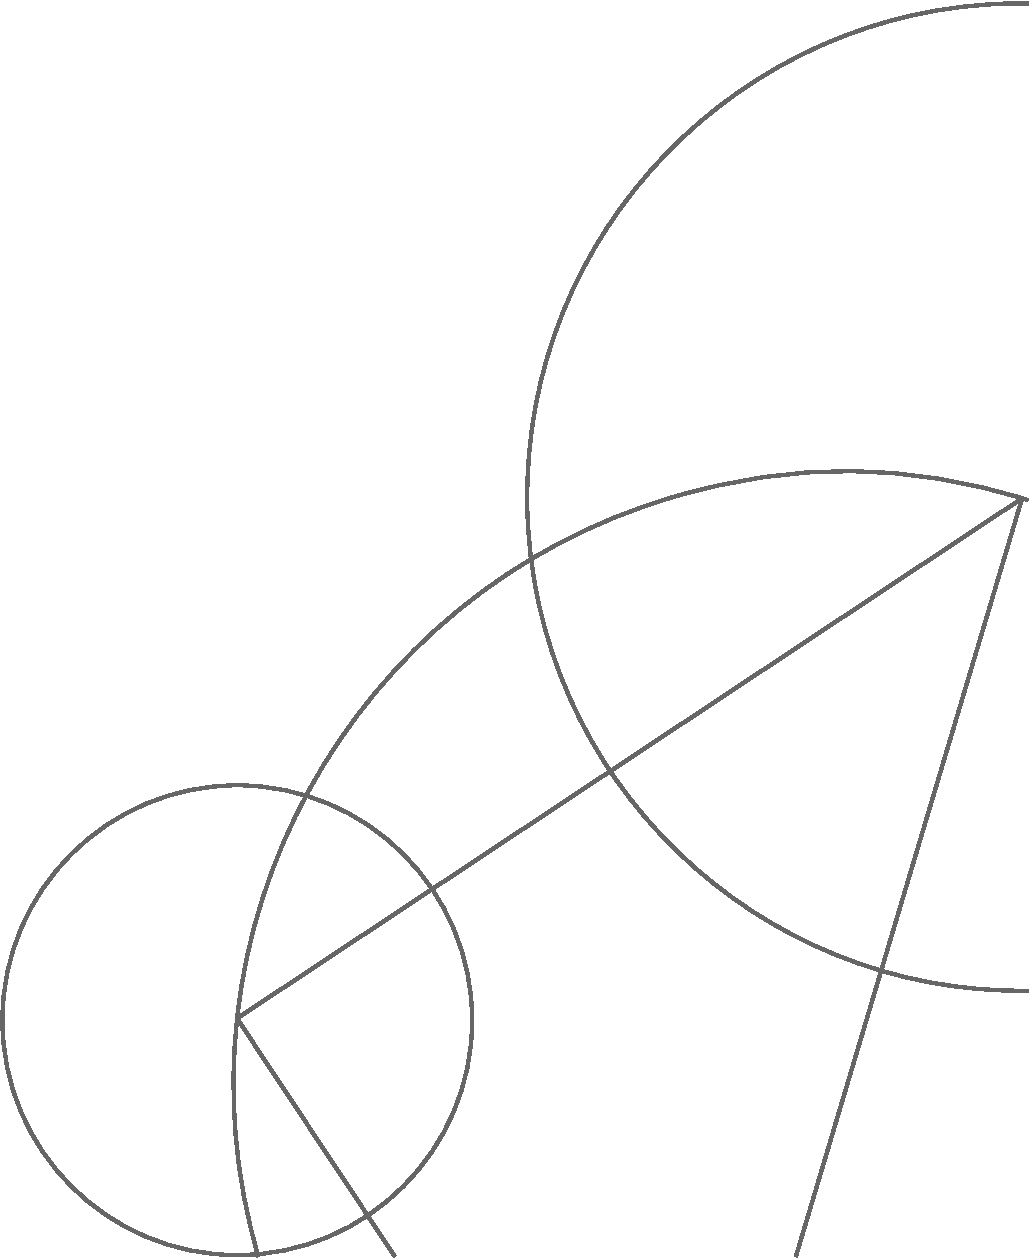
\includegraphics[height=75mm, keepaspectratio]{ku/grid}
    \end{textblock*}


    \begin{textblock*}{0mm}(115mm , 5mm)
        
\includegraphics[height=13mm, keepaspectratio]{ku/logo}
    \end{textblock*}

    %\begin{textblock*}{0mm}(82mm , 7mm)
    %    
\includegraphics[height=7mm, keepaspectratio]{ku/cic}
    %\end{textblock*}

    \begin{textblock*}{200mm}(-12mm, 17.0mm)
        \textblockcolour{kured}
        \fontsize{0}{0}\selectfont
        \TPMargin{0mm}
        \vspace{0.1mm}.
    \end{textblock*}

    \begin{textblock*}{0mm}(0mm,-1mm)
        
\includegraphics[height=15mm, keepaspectratio]{ku/corner}
    \end{textblock*}

    \begin{textblock*}{115mm}(17mm, 13mm)
        \textblockcolour{}
        \fontsize{8.5}{12}\selectfont
        \textcolor{kugray}{Faculty of Science}
    \end{textblock*}

    \begin{textblock*}{75mm}(17mm, 35mm)
        \textblockcolour{}

        \fontsize{10.5}{14}\selectfont
        \textcolor{kured}{\inserttitle}\par
        \bigskip
        \fontsize{8.5}{12}\selectfont
        \insertauthor\par
        \insertdate\par

  \end{textblock*}
}

\setbeamertemplate{footline}{
    \ifnum\c@framenumber>1

        \begin{textblock*}{4mm}(125mm, 94mm)
            \textblockcolour{}
            \fontsize{5.5}{6}\selectfont
            \textcolor{kugray}{\textmd{\insertframenumber}}
        \end{textblock*}

    \fi
}


\makeatother

\title{
  Regular Expression Matching In Genomic Data \\
  \textcolor{black}{\tiny{Translating scan\_for\_matches Patterns into Regular Expressions}}
}
%\author{Rasmus Haarslev\\ Troels Thomsen}
%\institute{ShareLaTeX}
\date{}

\begin{document}

\frame{\titlepage}

\begin{frame}
    \frametitle{Scan\_for\_matches programmet}
    
    \begin{itemize}
   		\item Fuzzy matching i genomisk data med mismatches, insertions og deletions.
   		\item Range matching
   		\item Reverse compliment
   		\item Genbrugelige matches
   		\item \texttt{p1=AGCTCTCCGTAACGGA[1,0,0] 4...8 {\raise.17ex\hbox{$\scriptstyle\mathtt{\sim}$}}p1}
	\end{itemize}    
   
\end{frame}

\begin{frame}
	\frametitle{Regular expressions oversættelse}
	
	\begin{itemize}
		\item \texttt{4...8} : \.{4,8}
		\item \texttt{AGCT[1,0,0]} : \texttt{(?i)(?:(?:AGCT)|
		(?:AGC[\^{}TN])|(?:AG[\^{}CN]T)|
		(?:A[\^{}GN]CT)|(?:[\^{}AN]GCT))(?-i)}
		\item Ingen gemte matches for ranges.
	\end{itemize}
\end{frame}

\begin{frame}
	\frametitle{Vores algoritme til oversættelse}
	
\begin{algorithm}[H]
\tiny
  	\begin{algorithmic}[1]
		\Function{find\_combinations}{$seq$, $m_{max}$, $d_{max}$, $i_{max}$}
    		\If{$seq.length > 1$}
    			\Let{left\_tree}{\Call{find\_combinations}{seq[0..(seq.length/2).floor-1], $m_{max}$, $i_{max}$, $d_{max}$}} \label{alg:divide:leftT}
    			\Let{right\_tree}{\Call{find\_combinations}{seq[(seq.length/2).floor..-1], $m_{max}$, $i_{max}$, $d_{max}$}} \label{alg:divide:rightT}
    		\Else
    			\Returns{List of all mismatch, insertion, and deletion combinations of seq} \label{alg:divide:conquer}
    		\EndIf
    		\State
    		\Let{combined}{empty list}
    		\Let{unique\_combinations}{empty set}
    		\ForAll{LL \In left\_tree} \Comment{LL: Left leaf}
    			\ForAll{RL \textbf{in} right\_tree} \label{alg:divide:inner} \Comment{RL: Right leaf}
    				\If{$LL.m + RL.m > m_{max}$ \Or $LL.d + RL.d > d_{max}$ \Or $LL.i + RL.i > i_{max}$} \label{alg:divide:invariant1}
    					\State continue
    				\EndIf
    				\If{\Not LL.seq + RL.seq \In unique\_combinations.keys} \label{alg:divide:invariant2}
    					\Let{unique\_combinations}{LL.seq + RL.seq}
    					\Let{combined}{LL + RL}
    				\EndIf
    			\EndFor
    		\EndFor
    		\Returns{combined}
    		\EndFunction
  	\end{algorithmic}
\end{algorithm}

\end{frame}

\begin{frame}
	\frametitle{Algoritme eksempel}
	Oversæt \texttt{AGCT[1,0,0]} til regular expressions
\end{frame}

\begin{frame}
	\frametitle{Algoritme eksempel}
	
	\begin{center}
	\begin{tikzpicture}[->,>=stealth', level/.style={sibling distance = 5cm, level distance = 1.5cm}, scale=0.6,transform shape]
    \node [treenode] {AGCT}
    child
    {
        node [treenode] {AG}
    }
    child
    {
    		node [treenode] {CT}
    }
;
	\end{tikzpicture}
	\end{center}
	
\end{frame}

\begin{frame}
	\frametitle{Algoritme eksempel}
	
	\begin{center}
	\begin{tikzpicture}[->,>=stealth', level/.style={sibling distance = 5cm, level distance = 1.5cm}, scale=0.6,transform shape]
    \node [treenode] {AGCT}
    child
    {
        node [treenode] {AG} 
        child
        {
            node [treenode, xshift=1cm] {A} 
        }
      	child
        {
        		node [treenode, xshift=-1cm] {G}
        }
    }
    child
    {
    		node [treenode] {CT}
    		child
        {
            node [treenode, xshift=1cm] {C} 
        }
        child
        {
        		node [treenode, xshift=-1cm] {T}
        }
    }
;
	\end{tikzpicture}
	\end{center}
	
\end{frame}

\begin{frame}
	\frametitle{Algoritme eksempel}
	
	\begin{center}
	\begin{tikzpicture}[->,>=stealth', level/.style={sibling distance = 5cm, level distance = 1.5cm}, scale=0.6,transform shape]
    \node [treenode] {}
    child
    {
        node [treenode] {} 
        child
        {
            node [treenode, xshift=1cm] {[A, \_]} 
        }
      	child
        {
        		node [treenode, xshift=-1cm] {[G, \_]}
        }
    }
    child
    {
    		node [treenode] {}
    		child
        {
            node [treenode, xshift=1cm] {C} 
        }
        child
        {
        		node [treenode, xshift=-1cm] {T}
        }
    }
;
	\end{tikzpicture}
	\end{center}
	
\end{frame}

\begin{frame}
	\frametitle{Algoritme eksempel}
	
	\begin{center}
	\begin{tikzpicture}[->,>=stealth', level/.style={sibling distance = 5cm, level distance = 1.5cm}, scale=0.6,transform shape]
    \node [treenode] {}
    child
    {
        node [treenode] {[AG]} 
        child
        {
            node [treenode, xshift=1cm] {[A, \_]} 
        }
      	child
        {
        		node [treenode, xshift=-1cm] {[G, \_]}
        }
    }
    child
    {
    		node [treenode] {}
    		child
        {
            node [treenode, xshift=1cm] {C} 
        }
        child
        {
        		node [treenode, xshift=-1cm] {T}
        }
    }
;
	\end{tikzpicture}
	\end{center}
	
\end{frame}

\begin{frame}
	\frametitle{Algoritme eksempel}
	
	\begin{center}
	\begin{tikzpicture}[->,>=stealth', level/.style={sibling distance = 5cm, level distance = 1.5cm}, scale=0.6,transform shape]
    \node [treenode] {}
    child
    {
        node [treenode] {[AG, A\_]} 
        child
        {
            node [treenode, xshift=1cm] {[A, \_]} 
        }
      	child
        {
        		node [treenode, xshift=-1cm] {[G, \_]}
        }
    }
    child
    {
    		node [treenode] {}
    		child
        {
            node [treenode, xshift=1cm] {C} 
        }
        child
        {
        		node [treenode, xshift=-1cm] {T}
        }
    }
;
	\end{tikzpicture}
	\end{center}
	
\end{frame}

\begin{frame}
	\frametitle{Algoritme eksempel}
	
	\begin{center}
	\begin{tikzpicture}[->,>=stealth', level/.style={sibling distance = 5cm, level distance = 1.5cm}, scale=0.6,transform shape]
    \node [treenode] {}
    child
    {
        node [treenode] {[AG, A\_, \_G]} 
        child
        {
            node [treenode, xshift=1cm] {[A, \_]} 
        }
      	child
        {
        		node [treenode, xshift=-1cm] {[G, \_]}
        }
    }
    child
    {
    		node [treenode] {}
    		child
        {
            node [treenode, xshift=1cm] {C} 
        }
        child
        {
        		node [treenode, xshift=-1cm] {T}
        }
    }
;
	\end{tikzpicture}
	\end{center}
	
\end{frame}

\begin{frame}
	\frametitle{Algoritme eksempel}
	
	\begin{center}
	\begin{tikzpicture}[->,>=stealth', level/.style={sibling distance = 5cm, level distance = 1.5cm}, scale=0.6,transform shape]
    \node [treenode] {}
    child
    {
        node [treenode] {[AG, A\_, \_G]} 
        child
        {
            node [treenode, xshift=1cm] {[A, \_]} 
        }
      	child
        {
        		node [treenode, xshift=-1cm] {[G, \_]}
        }
    }
    child
    {
    		node [treenode] {[CT, C\_, \_T]}
    		child
        {
            node [treenode, xshift=1cm] {[C, \_]} 
        }
        child
        {
        		node [treenode, xshift=-1cm] {[T, \_]}
        }
    }
;
	\end{tikzpicture}
	\end{center}
	
\end{frame}

\begin{frame}
	\frametitle{Algoritme eksempel}
	
	\begin{center}
	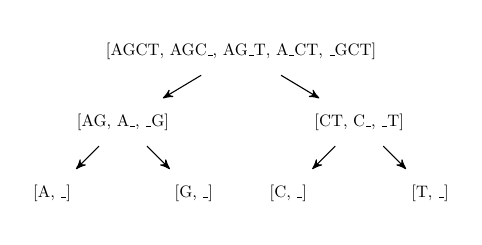
\begin{tikzpicture}[->,>=stealth', level/.style={sibling distance = 5cm, level distance = 1.5cm}, scale=0.6,transform shape]
    \node [treenode] {[AGCT, AGC\_, AG\_T, A\_CT, \_GCT]}
    child
    {
        node [treenode] {[AG, A\_, \_G]} 
        child
        {
            node [treenode, xshift=1cm] {[A, \_]} 
        }
      	child
        {
        		node [treenode, xshift=-1cm] {[G, \_]}
        }
    }
    child
    {
    		node [treenode] {[CT, C\_, \_T]}
    		child
        {
            node [treenode, xshift=1cm] {[C, \_]} 
        }
        child
        {
        		node [treenode, xshift=-1cm] {[T, \_]}
        }
    }
;
	\end{tikzpicture}
	\end{center}
	
\end{frame}

\end{document}